\documentclass[11pt, oneside]{article}   	% use "amsart" instead of "article" for AMSLaTeX format
\usepackage[margin = 1in]{geometry}                		% See geometry.pdf to learn the layout options. There are lots.
\geometry{letterpaper}                   		% ... or a4paper or a5paper or ... 
%\geometry{landscape}                		% Activate for rotated page geometry
%\usepackage[parfill]{parskip}    		% Activate to begin paragraphs with an empty line rather than an indent
\usepackage{graphicx}				% Use pdf, png, jpg, or eps§ with pdflatex; use eps in DVI mode
								% TeX will automatically convert eps --> pdf in pdflatex		
\usepackage{amssymb}
\usepackage{amsmath}
\usepackage[shortlabels]{enumitem}
\usepackage{float}
\usepackage{tikz-cd}
\usepackage{subcaption}
\usepackage{slashed}

\usepackage{amsthm}
\theoremstyle{definition}
\newtheorem{definition}{Definition}[section]
\newtheorem{theorem}{Theorem}[section]
\newtheorem{corollary}{Corollary}[theorem]
\newtheorem{lemma}[theorem]{Lemma}

\newcommand{\N}{\mathbb{N}}
\newcommand{\R}{\mathbb{R}}
\newcommand{\Z}{\mathbb{Z}}
\newcommand{\Q}{\mathbb{Q}}

\usepackage{simpler-wick}
\usepackage[compat=1.0.0]{tikz-feynman}   %note you need to compile this in LuaLaTeX for diagrams to render correctly

% make arrow superscripts
\DeclareFontFamily{OMS}{oasy}{\skewchar\font48 }
\DeclareFontShape{OMS}{oasy}{m}{n}{%
         <-5.5> oasy5     <5.5-6.5> oasy6
      <6.5-7.5> oasy7     <7.5-8.5> oasy8
      <8.5-9.5> oasy9     <9.5->  oasy10
      }{}
\DeclareFontShape{OMS}{oasy}{b}{n}{%
       <-6> oabsy5
      <6-8> oabsy7
      <8->  oabsy10
      }{}
\DeclareSymbolFont{oasy}{OMS}{oasy}{m}{n}
\SetSymbolFont{oasy}{bold}{OMS}{oasy}{b}{n}

\DeclareMathSymbol{\smallleftarrow}     {\mathrel}{oasy}{"20}
\DeclareMathSymbol{\smallrightarrow}    {\mathrel}{oasy}{"21}
\DeclareMathSymbol{\smallleftrightarrow}{\mathrel}{oasy}{"24}
%\newcommand{\cev}[1]{\reflectbox{\ensuremath{\vec{\reflectbox{\ensuremath{#1}}}}}}
\newcommand{\vecc}[1]{\overset{\scriptscriptstyle\smallrightarrow}{#1}}
\newcommand{\cev}[1]{\overset{\scriptscriptstyle\smallleftarrow}{#1}}
\newcommand{\cevvec}[1]{\overset{\scriptscriptstyle\smallleftrightarrow}{#1}}

\newcommand{\dbar}{d\hspace*{-0.08em}\bar{}\hspace*{0.1em}}

%SetFonts

%SetFonts


\title{Momentum Fraction NPR}
\author{Patrick Oare}
\date{}							% Activate to display a given date or no date

\begin{document}
\maketitle


\section{Renormalization in the RI'-MOM scheme}

We will renormalize a local operator $\mathcal O(z)$ in the RI'-MOM scheme~\cite{ri_mom}. To renormalize 
$\mathcal O$ at scale $\mu^2$ in this scheme, we impose that in a fixed gauge, the amputated three point 
function $\Gamma$ at incoming quark momentum $p^2 = \mu^2$ and current momentum $q = 0$ equals 
its tree level value at $p^2 = \mu^2$. 

Our notation will denote bare quantities as $A^{(0)}$, and renormalized quantities with a $R$ subscript, when appropriate. 
The lattice parameter will be denoted $a$ and the size of the lattice in the $\mu$ direction is $L_\mu$. 
We will work with momentum scales:
\begin{equation}
	\tilde p_\mu\equiv \frac{2}{a}\sin\left(\frac{\pi a}{L_\mu} k_\mu\right) \;\;\;\;\;\;\;\;\;\;\;\;\;\;\;\;\;\;\;\;\;\;\;\;\;\;\;\;\;\;\;\;\;\;\;\;\;\;\;\;\;\;\;\;\;\;\;\;
	p_\mu\equiv \frac{2\pi}{L_\mu} k_\mu
\end{equation}
where $\tilde p$ is the lattice momentum and $p$ is the linear momentum for mode $k\in\mathbb Z^4$. We will work in Landau gauge, 
where the gauge parameter is set to $\tau = 0$. 

On the lattice we must directly compute the propagator $S^{(0)}(p^2)$ and the bare three point function $G^{(0)}(p^2)$, defined as:
\begin{align}
	S^{(0)}(p^2) &\equiv \frac{1}{V}\sum_{x, y} e^{ip\cdot (x - y)}\langle q(x) \overline q(y)\rangle ~\label{eq:prop} \\
	G^{(0)}(p^2) &\equiv \frac{1}{V}\sum_{x, y, z}e^{ip\cdot (x - y)}\langle q(x)\mathcal O(z) \overline{q}(y)\rangle~\label{eq:green}
\end{align}
i.e. we are projecting the source and sink to a definite momentum and projecting the operator $\mathcal O(z)$ to zero 
momentum. 

We define the renormalized operator and quark fields to be:
\begin{align}
	\mathcal O_R(\mu) &\equiv \mathcal Z(\mu) \,\mathcal O^{(0)} ~\label{eq:zo_def} \\
	q_R(\mu) &\equiv \sqrt{\mathcal Z_q(\mu)} q^{(0)}~\label{eq:zq_def}
\end{align}
where $\mathcal O_R(\mu)$ is our renormalized operator, $\mathcal Z(\mu)$ is the renormalization coefficient of 
interest, and $\mathcal O^{(0)}$ is the lattice (bare) operator.

In the RI'-MOM scheme the quark field renormalization $\mathcal Z_q$ is defined to be:
\begin{equation}
	\mathcal Z_q(p^2)|_{\tilde p^2 = -\mu_R^2} = i\frac{1}{12\tilde p^2}tr\left\{S^{-1}(\tilde p^2)\slashed{\tilde p}\right\}\bigg|_{p^2 = \mu^2} = \left[\frac{tr\left\{i\sum_{\nu = 1}^4 \gamma_\nu \sin(ap_\nu) a S(p^2)^{-1}\right\}}{12\sum_{\nu = 1}^4 \sin^2(ap_\nu)}\right]_{p^2 = \mu^2}~
	\label{eq:quark_renorm}
\end{equation}
The twelve is a normalization for the number of color and number of spin indices, which we will see in many of the expressions. 
Note that this may differ by a negative sign from other references, as we are using the phase convention $e^{ip\cdot(x - y)}$ 
for our momentum projection in Equations~\ref{eq:prop} and~\ref{eq:green}.

Let $\Gamma$ be the \textbf{amputated three point function}, bare or renormalized. $\Gamma$ can be defined in 
terms of the propagator $S(p^2)$ and three point function $G(p^2)$ as:
\begin{equation}
	\Gamma(p^2) = S(p^2)^{-1} G(p^2) S(p^2)^{-1}
\end{equation}
By using the definitions~\ref{eq:zo_def} and~\ref{eq:zq_def} we can see that $G_R(p^2) = \mathcal{Z}_q\mathcal Z_\mathcal{O} G^{(0)}(p^2)$ 
and $S_R(p^2) = \mathcal{Z}_q S^{(0)}(p^2)$, hence we can relate the renormalized $\Gamma_R$ to the bare 
$\Gamma^{(0)}$ which is computed on the lattice:
\begin{equation}
	\Gamma_R(p^2) = \mathcal{Z}_q(\mu^2)^{-1} \mathcal Z_\mathcal{O}(\mu^2) \Gamma^{(0)}(p^2)
\end{equation}

We can now apply the renormalization condition and define that $\Gamma_R(\tilde p^2)$ equals its tree level value $\Gamma_B(\tilde p^2)$ 
at the renormalization point $\tilde p^2 = \mu^2$:
\begin{equation}
	\bigg[\frac{\mathcal{Z}_\mathcal{O}(\tilde p^2)}{\mathcal{Z}_q(\tilde p^2)} \Gamma^{(0)}(\tilde p^2)\bigg]_{\tilde p^2 = \mu^2} = \Gamma_B(\tilde p^2 = \mu^2)~
	\label{eq:rc}
\end{equation}

\section{Isospin operator}

We will now specify the RI'-MOM method to our operator $\mathcal O^i(z) = \mathcal O^i_u(z) - \mathcal O^i_d(z)$, 
where the quark operators $\{\mathcal O^i_q\}_{i = 1}^3$ are basis elements of the tensor operator
\begin{equation}
	\mathcal T_{\mu\nu}^q(z)\equiv \overline q(z)\gamma_{\{\mu}\cevvec{D}_{\nu\}} q(z)
\end{equation}
in the irreducible representation $\tau_1^{(3)}$ of the hypercubic group $H(4)$. Here $\cevvec D = \vec D - \cev D$ is the 
antisymmetrized covariant derivative and the symmetric and traceless component of a tensor is defined to be:
\begin{equation}
	a_{\{\mu}b_{\nu\}} \equiv \frac{1}{2}(a_\mu b_\nu + a_\nu b_\mu) - \frac{1}{4}a_\alpha b^\alpha g_{\mu\nu}
\end{equation} 

We now must determine the tree level structure of this operator, and then perform a lattice computation to determine 
$\Gamma^{(0)}(\tilde p^2$ and $\mathcal Z_q(\tilde p^2)$. 

\subsection{Tree level structure of $\mathcal T$}

We begin by determining the amputated three point function for this operator at tree level $\Gamma_B(p^2)$, closely following 
the method in~\cite{sergey}. When $\mathcal T_{\mu\nu}$ is put on the lattice, its tree level value is proportional to two tensor 
structures:
\begin{align}
	i\Lambda_{\mu\nu}^{1}(\tilde p) &\equiv \frac{1}{2}(\tilde p_\mu \gamma_\nu + p_\nu \gamma_\mu) - \frac{1}{4} \slashed{\tilde p} \delta_{\mu\nu} \\
	i\Lambda_{\mu\nu}^2(\tilde p) &\equiv \frac{\tilde p_\mu \tilde p_\nu}{p^2} \slashed{\tilde p} - \frac{1}{4} \slashed{\tilde p} \delta_{\mu\nu}
\end{align}
In the continuum, $\mathcal T_{\mu\nu}$ is directly propotional to just $\Lambda^{(1)}_{\mu\nu}$, and we would not have 
to consider any mixing between these tensor structures. On the lattice, $\Lambda_{\mu\nu}^{(2)}$ comes in as a $\mathcal O(a)$ 
correction. To account for this mixing directly, we must redefine the renormalization condition in Equation~\ref{eq:rc}. We
expand the amputated Green's function $\Gamma(p)$. If we let $\Gamma^D(p) := \frac{1}{3} tr_C\{\Gamma(p)\}$ be the 
Dirac components of $\Gamma(p)$, then this expansion amounts to imposing the renormalization condition:
\begin{equation}
	\bigg[\Gamma_{\mu\nu}^D(\tilde p^2)\bigg]_{\tilde p^2 = \mu^2} = \Pi^1(\tilde p^2) \Lambda^1_{\mu\nu}(\tilde p^2) + \Pi^2(\tilde p^2) \Lambda^2_{\mu\nu}(\tilde p^2)~
	\label{eq:mix_rc}
\end{equation}
where $\Pi^1(\tilde p^2)$ and $\Pi^2(\tilde p^2)$ are coefficients which are related to the renormalization coefficients by:
\begin{equation}
	\Pi^i(\tilde p^2 = \mu^2) = \frac{Z_q}{Z_i(\tilde p^2 = \mu^2)}
\end{equation}
We will extract the renormalization coefficient proportional to the continuum tree level piece, 
$\mathcal Z_\mathcal{O}\equiv \mathcal Z_1$. 

To solve Equation~\ref{eq:mix_rc} for the $\Pi^i$, we construct a linear functional on the space of Dirac and Lorentz matrices 
by defining a form $\langle\cdot, \cdot\rangle$ whose action is:
\begin{equation}
	\langle \lambda^1, \lambda^2\rangle := \sum_{i\in\mathfrak R} tr_D\left\{\lambda^1_i \lambda^2_i\right\}
\end{equation}
where $\lambda^1, \lambda^2$ are objects with two Dirac and two Lorentz indices. Here, $\mathfrak R$ denotes the irrep 
of $H(4)$ that we are working in, which in our case is $\mathfrak R = \tau_1^{(3)}$. 
This form therefore sums over the normalized basis elements of the irrep:
\begin{align}
	\tau_1^{(3)} = span\bigg\{ &\frac{1}{\sqrt{2}} \left(\mathcal O_{\{33\}} - \mathcal O_{\{44\}}\right), \\ 
	& \frac{1}{\sqrt{2}} \left(\mathcal O_{\{11\}} - \mathcal O_{\{22\}}\right), \\
	& \frac{1}{2} \left(\mathcal O_{\{11\}} + \mathcal O_{\{22\}} - \mathcal O_{\{33\}} - \mathcal O_{\{44\}}\right) \bigg\}
\end{align}

We apply the functionals $\langle\Lambda^1, \cdot\rangle$ and $\langle\Lambda^2, \cdot\rangle$ to 
Equation~\ref{eq:mix_rc} to obtain the following system of equations which we can use to solve for the 
coefficients $\Pi^1$ and $\Pi^2$:
\begin{equation}
	\mathcal A^{ab}\Pi^b = \begin{pmatrix} \langle \Lambda^1, \Gamma(p) \rangle \\ \langle \Lambda^2, \Gamma(p) \rangle \end{pmatrix}
\end{equation}
where $\mathcal A^{ab}$ is the matrix of inner products:
\begin{equation}
	\mathcal A^{ab} \equiv \langle \Lambda^a, \Lambda^b\rangle
\end{equation}
where $a, b$ range over $1$ and $2$. Using the explicit form for $\Lambda^1$ and $\Lambda^2$, the matrix 
$\mathcal A^{ab}$ can be computed directly using the identities $tr\{\gamma_\mu\gamma_\nu\} = 4\delta_{\mu\nu}$, 
$(\slashed k)^2 = k^2$, and $tr\{1\} = 4$. The result is:
\begin{equation}
	\mathcal A^{ab}(\tilde p) = \begin{pmatrix} 3\tilde p^2 & \frac{1}{\tilde p^2} \left( -3 \tilde p^{[4]} + 2 \sum_{i < j} \tilde p_i^2 \tilde p_j^2\right) \\ \frac{1}{\tilde p^2} 
	\left( -3 \tilde p^{[4]} + 2 \sum_{i < j} \tilde p_i^2 \tilde p_j^2\right) & \frac{1}{\tilde p^2} \left( -3 \tilde p^{[4]} + 2 \sum_{i < j} \tilde p_i^2 \tilde p_j^2\right) \end{pmatrix}
\end{equation}
where $p^{[4]}$ is the hypercubic invariant $\sum_i p_i^4$. We invert this matrix at each lattice momentum $\tilde p_\mu$ used in our 
computation to solve for the $\Pi^i$ coefficients, and hence $\mathcal Z_{\mathcal O}$. 

\subsection{Lattice computation}

We now turn our attention to computing the bare Green's functions $S^{(0)}(\tilde p^2)$ and $G^{(0)}(\tilde p^2)$. 
As in~\cite{gockeler}, we expand the diagonal components of our operator as:
\begin{equation}
	\sum_z\mathcal T^q_{\mu\mu}(z) = \sum_{z, z'}\overline q(z)\, J_\mu(z, z')\,q(z')~
	\label{eq:operator_mom_proj}
\end{equation}
Using the definition of the derivatives:
\begin{align}
	\vec D\psi(z) &= \frac{1}{2}\left(U_\mu(z)\psi(z + \hat\mu) - U_\mu(n - \hat\mu)^\dagger \psi(z - \hat\mu)\right) \\
	\overline\psi(z) \cev D &= \frac{1}{2}\left(\overline\psi(z + \hat\mu)U_\mu(z)^\dagger - 
	\overline\psi(z - \hat\mu) U_\mu(z - \hat\mu)\right)
\end{align}
we find the current $J_\mu(z, z')$ is:
\begin{equation}
	J_\mu(z, z') = \left[U_\mu(z) \delta_{z + \hat\mu, z'} - U_\mu(z')^\dagger\delta_{z - \hat\mu, z'}\right]\gamma_\mu
\end{equation}

For the up-down quark operator difference $\mathcal T_\mu\equiv\mathcal T_\mu^u - \mathcal T_{\mu\mu}^d$, we use 
Equation~\ref{eq:operator_mom_proj} to expand:
\begin{equation}
	\sum_z \mathcal T_\mu(z) = \sum_{z, z'}\left[\overline u(z)\, J_\mu(z, z')\, u(z') - \overline d(z)\, J_\mu(z, z')\, d(z')\right]
\end{equation}
Plugging this into Equation~\ref{eq:green}, we find that we can expand the total up quark Green's function (here $\alpha, 
\beta$ are Dirac indices) as:
\begin{equation}
	G^{\alpha\beta}(p) = \frac{1}{\sqrt 2}\left(G_3^{\alpha\beta}(p) - G_4^{\alpha\beta} (p)\right)
\end{equation}
where:
\begin{align}
	G_\mu^{\alpha\beta}(p) &= \frac{1}{V}\sum_{x, y, z} e^{-ip(x - y)}\langle u^\alpha(x)\mathcal T_\mu(z) \overline u^\beta(y)
	\rangle \\
	&= \frac{1}{V}\sum_{x, y, z, z'} e^{-ip(x - y)}\left[\langle u^\alpha(x)\overline u^\sigma(z) J_\mu^{\sigma\rho}(z, z') 
	u(z')^\rho\overline u^\beta(y)\rangle - \langle u^\alpha(x)\overline d^\sigma(z) J_\mu^{\sigma\rho}(z, z') d^\rho(z') 
	\overline u^\beta(y)\rangle 
	\right]
\end{align}
Now we perform all possible Wick contractions on the matrix elements to write them as propagators:
\begin{align}
	\langle u^\alpha(x)\overline u^\sigma(z) &J_\mu^{\sigma\rho}(z, z') u^\rho(z')\overline u^\beta(y)\rangle = 
	\langle \wick{
		\c1 u \c1{\overline u} J \c2 u \c2{\overline u}
	} \rangle + \langle \wick{
		\c1 u \c2{\overline u} J \c2 u \c1{\overline u} 
	} \rangle \nonumber \\ 
	&= S^{\alpha\sigma}(x, z) J^{\sigma\rho}_\mu(z, z') S^{\rho\beta}(z', y) + (-1)^3 S^{\alpha\beta}(x, y) 
	J^{\sigma\rho}_\mu(z, z')S^{\rho\sigma}(z', z) \\
	\nonumber\\
	\langle u^\alpha(x)\overline d^\sigma(z) &J_\mu^{\sigma\rho}(z, z') d^\rho(z') \overline u^\beta(y)\rangle = 
	\langle \wick{
		\c1 u \c2{\overline d} J \c2 d \c1{\overline u}
	}\rangle\nonumber \\ 
	&= (-1)^3 S^{\alpha\beta}(x, y) J^{\sigma\rho}_\mu(z, z')S^{\rho\sigma}(z', z)
\end{align}
where the factors of $(-1)$ come from rearranging the contraction so that the contracted pieces are of the form 
$\langle u\overline u\rangle$. The vacuum pieces cancel because the up and down quark propagators are degenerate, so the 
final result is very clean:
\begin{equation}
	G_\mu(p) = \frac{1}{V}\sum_{x, y, z, z'}e^{ip(x - y)} S(x, z) J_\mu (z, z') S(z', y)~
	\label{eq:greens_function}
\end{equation}
This is our central equation, but note that computing this directly on the lattice would involve computing the two point 
propagator $S(x, y)$ at each two points on the lattice. This is much too computationally intensive, so we must resort to 
other techniques to accomplish this. 

There are two primary ways to compute this on the lattice.
We can compute this directly using momentum sources, or 
we can use the sequential source technique. Momentum sources work specifically for Equation~\ref{eq:greens_function}, 
but produce a significantly better signal on a small number of configurations. On the other hand, sequential source 
is much more general, but produces more noise. We will discuss each method below.
%either compute this \textbf{through the operator} or 
%\textbf{through the sink}, and below we will discuss each method and the pros and cons of each. 

\subsection{Momentum sources}

Observe that we can rewrite Equation~\ref{eq:greens_function} as:
\begin{align}
	G_\mu(p) &= \frac{1}{V}\sum_{x, y, z, z'} e^{ipx} S(x, z) J_\mu(z, z') e^{-ipy} S(z', y) \nonumber\\
	&= \frac{1}{V}\sum_{z, z'}\gamma_5\left(\sum_x S(z, x) e^{-ipx}\right)^\dagger\gamma_5 J_\mu(z, z') \left(\sum_y S(z', y) 
	e^{-ipy} \right) \nonumber\\
	&= \frac{1}{V}\sum_{z, z'} \gamma_5 \tilde S_p(z)^\dagger \gamma_5 J_\mu(z, z') \tilde S_p(z')~
	\label{eq:through_sink}
\end{align}
where we have defined $\tilde S_p(z)$ as:
\begin{equation}
	\tilde S_p(z) = \sum_x S(z, x) e^{-ipx}
\end{equation}

The advantage of casting the equation in this form is that we can solve for $\tilde S_p(z)$ directly by inverting the Dirac 
equation with a momentum source, i.e. we have:
\begin{equation}
	\sum_{z} D(x, z) \tilde S_p(z) = e^{-ipx}
\end{equation}
where $D(x, z)$ is the Dirac operator. This means that upon solving for $\tilde S_p(z)$ and plugging this into 
Equation~\ref{eq:through_sink}, we can solve directly for $G_\mu(p)$. 

We can also use the propagator we get from the momentum source inversion to directly compute the propagator 
in Equation~\ref{eq:mom_prop} as follows:
\begin{equation}
	S(p) = \frac{1}{V}\sum_{x, y} e^{ip\cdot (x - y)} S(x, y) = \frac{1}{V}\sum_x e^{ip\cdot x} \tilde S_p(x) 
\end{equation}

This is an exact equation and it does not rely on translational invariance in the infinite statistics limit. 
Therefore, this method will give much better signal and can be run efficiently on a small number of configurations. The 
downside to this is that we require a propagator inversion for each choice of sink momentum. 
To compute $G(p)$ for a large number of sink momenta, as we need to do to extrapolate $\mathcal Z(\mu)$ in the 
continuum limit, a propagator inversion at each sink momenta is not feasible. We must instead choose the sink momentum 
wisely to be able to extract the discretization artifacts and extrapolate $\mathcal Z(\mu)$ to the continuum, which we will 
describe in Section~\ref{sec:artifacts}. 

\subsection{Sequential source method}

In practice we will use the sequential source method, which if implemented correctly does not force us to invert a propagator 
at every sink momenta. This technique is also much more general than the one previously described, but it suffers from 
more noise because it relies on the translational invariance of the lattice, which only exists in the infinite statistics 
limit. The idea of the sequential source method is that if we have an equation involving the full propagator $S(x, y)$, we can 
invert a source which depends on the propagator $S(x)$. For example, in this problem we wish to evaluate 
Equation~\ref{eq:greens_function}, but we cannot simply evaluate $S(x, y)$ for every $x$ and $y$. To get around this, 
consider using a source
\begin{equation}
	b(z) = \sum_{z'} J_\mu(z, z') S(z', 0)~
	\label{eq:source}
\end{equation}
to invert the Dirac equation, which will solve for $M(x)$ in this equation:
\begin{equation}
	\sum_x D(z, x) M(x) = b(z)
\end{equation} 
where $D(x, z)$ is the Dirac operator. Upon inversion, using that $\sum_z S(y, z) D(z, x) = \delta(y - x)$, we can move the 
Dirac operator to the other side as $D^{-1}(y, z) = S(y, z)$ and obtain:
\begin{equation}
	M(x) = \sum_z D^{-1}(x, z) b(z) = \sum_{z, z'} S(x, z) J_\mu(z, z') S(z', 0)~
	\label{eq:inversion}
\end{equation}
Note that we have summed the full propagator $S(x, z)$ for the price of a single inversion of the source $b(z)$. We can then 
reconstruct Equations~\ref{eq:mom_prop} and~\ref{eq:greens_function} for the momentum-projected Green's function 
and propagator in the infinite statistics limit when translational invariance is restored:
\begin{align}
	G_\mu(p)\approx \frac{1}{V} \sum_x e^{ipx} M(x) &= \frac{1}{V} \sum_{x, z, z'} e^{ipx} S(x, z) J_\mu(z, z') S(z', 0) \\
		S(p)&\approx\frac{1}{V}\sum_x e^{ipx} S(x, 0)
\end{align}

We can improve the performance of this by randomly sampling $N$ lattice points to approximate the sums over $y$ in 
our equations for $S(p)$ and $G(p)$. If we sample the points $\{y_i\}_{j = 1}^N$, then we can make the replacement 
$\sum_y\mapsto \frac{V}{N}\sum_j$, and so we have:
\begin{align}
	G_\mu(p)&\approx \frac{1}{N}\sum_{x, z, z'}\sum_j e^{ip(x - y_j)} S(x, z) J_\mu(z, z') S(z', y_j) \\
	S(p) &\approx \frac{1}{N} \sum_x\sum_j e^{ip\cdot(x - y_j)} S(x, y_j)
\end{align}

Since we are interested in renormalizing the operators in each irrep, we must take the operators we are measuring to be:
\begin{align}
	\mathcal O_1 &= \frac{1}{\sqrt{2}}\left(\mathcal T_{33} - T_{44}\right) \\
	\mathcal O_2 &= \frac{1}{\sqrt{2}}\left(\mathcal T_{11} - T_{22}\right) \\
	\mathcal O_3 &= \frac{1}{2}\left(\mathcal T_{11} + \mathcal T_{22} - \mathcal T_{33} - T_{44}\right)
\end{align}
which give us currents:
\begin{align}
	\mathcal J_1 &= \frac{1}{\sqrt{2}}(J_3 - J_4) \\
	\mathcal J_2 &= \frac{1}{\sqrt 2} (J_1 - J_2) \\
	\mathcal J_3 &= \frac{1}{2} (J_1 + J_2 - J_3 - J_4)
\end{align}
and we must compute the 3 propagators using $\mathcal J_i$ QLUA. 

To check an implementation of this method, we can invert a sequential propagator which depends on momentum. If we 
replace $S(z', 0)$ in Equation~\ref{eq:source} and invert, we find that:
\begin{align}
	b_\mu^{(p)}(z) &= \sum_{z'} J_\mu(z, z') \tilde S_p(z') = \sum_{z', y} e^{-ipy} J_\mu(z, z') S(z', y) \\
	M_\mu^{(p)}(x) &= \sum_{z} S(x, z) b_\mu^{(p)}(z) = \sum_{z, z', y} e^{-ipy} S(x, z) J_\mu(z, z') S(z', y)
\end{align}
When we momentum project to find the Green's function $G(p)$, this no longer relies on translation invariance and should 
match our result with the momentum inversion exactly:
\begin{equation}
	G_\mu(p) = \sum_x e^{ipx} M_\mu^{(p)}(x) = \sum_{x, y, z, z'} e^{ip(x - y)} S(x, z) J_\mu(z, z') S(z', y)
\end{equation}

In our case with a large amount of sink momenta, this method is much more robust than inverting a momentum source 
because we one inversion can give us $G(p)$ at every value of the sink momentum. We will call this construction going 
\textbf{through the operator}, because the inversion in Equation~\ref{eq:inversion} projects the current insertion onto $q = 0$ 
momentum. If we had been interested in projecting the operator onto different momentum values, then we would need to 
use a new sequential source (modify Equation~\ref{eq:source}) for each value of the operator momentum. Pictorially, we are 
inverting at the operator momentum, then tying up at the sink momentum. On the other hand, we reverse the direction of 
inversion and invert our propagator at each sink momentum first, then tie up the line at the operator. This method is called 
going \textbf{through the sink}. We can represent these different methods below, where in our case $q = 0$. 

In this problem inversion through the sink would require too many propagator inversions like in the previous momentum 
source method, and it would also be noisy like inversion through the operator. As such, there is no reason to consider it, 
and I included it here mainly for generality. 

Our result for the coefficient in the RI'-MOM scheme is plotted below.
\begin{figure}[H]
	\centering
	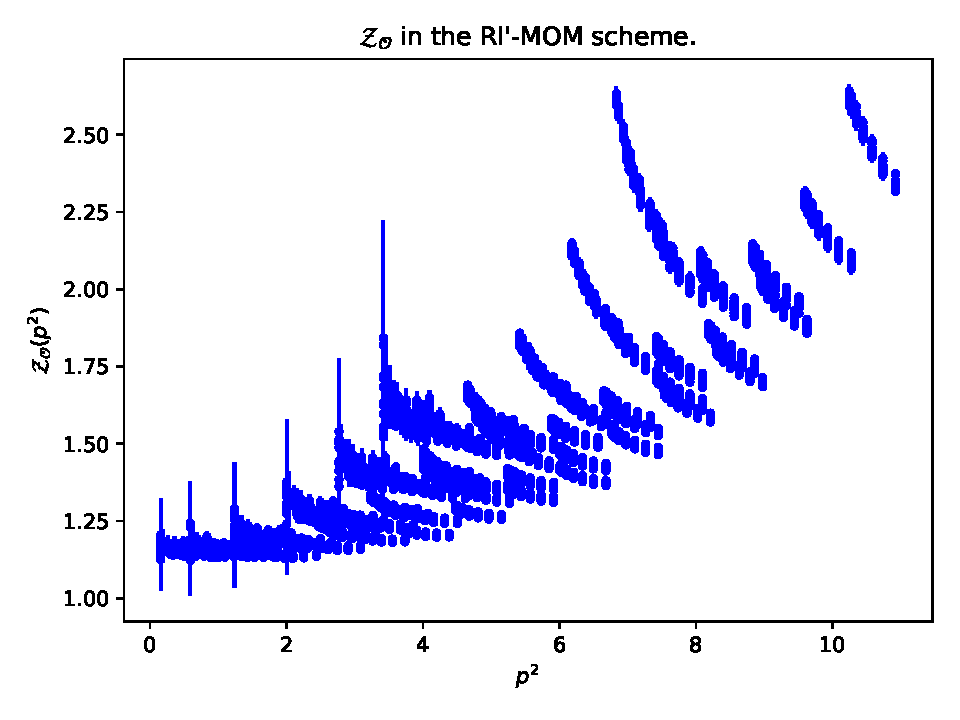
\includegraphics[width = .6\textwidth]{ZRIMOM}
	\caption{Renormalization coefficient for $\mathcal{Z}_{\mathcal{O}}$ in the RI'-MOM scheme.}
\end{figure}

\newpage
\section{Analysis}

\subsection{Matching to $\overline{MS}$}

To convert our results from RI'-MOM to $\overline{MS}$, we will use J.A. Gracey's results for the renormalization coefficients 
$\mathcal{Z}_\mathcal{O}$~\cite{gracey_zo} and $\mathcal{Z}_q$~\cite{gracey_zq}, computed using lattice perturbation theory both in the 
RI'-MOM and the $\overline{MS}$ schemes.

We will match our results to $\overline{MS}$ by converting them multiplicatively with the corresponding matching coefficient:
\begin{equation}
	C(\mu_0) \equiv \frac{\mathcal{Z}^{\overline{MS}}(\mu_0)}{\mathcal{Z}^{RI'-MOM}(\mu_0)}
\end{equation}
evaluated at the scale $\mu_0\equiv 2\;GeV$. This is done in two steps:
\begin{enumerate}
	\item Use the RI'-MOM anomalous dimension $\gamma$ to run $Z(\mu)$ to the matching scale $\mu_0$. 
	\item Convert to $\overline{MS}$ by multiplying with $C$.
\end{enumerate}

We will work through these two steps in detail for the renormalization coefficient $\mathcal Z_\mathcal{O}$. We begin 
by running the strong coupling $\alpha(\mu)$ to each renormalization point, as it needed to determine $\gamma$. 
This running is performed using the RunDec package~\cite{run_dec} to integrate the 3 loop beta function. We initialize 
the running at the scale of the $Z$ boson to be 
\begin{equation}
	\alpha(m_Z) = 0.119
\end{equation}
which has been determined by the Particle Data Group (PDG)~\cite{pdg}. We will also use the PDG for the mass of the 
$Z$-boson and the quark masses:
\begin{align}
	m_z &= 91.187\pm 0.0021 \textnormal{ GeV} & m_b = 4.18^{+0.03}_{-0.02}\textnormal{ GeV} \\
	m_c &= 1.27\pm 0.02\textnormal{ GeV} & m_s = 93^{+11}_{-5}\textnormal{ MeV}
\end{align}
We use the 5-flavor QCD beta function to flow $\alpha(m_Z)$ to $m_b$, then the 4-flavor beta function to flow $\alpha(m_b)$ to 
$m_c$, and finally use the 3 flavor beta function to determine $\alpha(\mu_0)$. For any renormalization scales $\mu < m_s$, 
we flow to $m_s$ using the 3 flavor beta function, then flow $\alpha(m_s)$ to the corresponding scale $\mu$ with 2 flavors. 
Our result for $\mu_0 = 2$ GeV is:
\begin{equation}
	\alpha(\mu_0 = 2 \textnormal{ GeV}) = 0.3069
\end{equation}

We are now in position to run $\mathcal Z_\mathcal{O}^{RI'-MOM}(\mu)$ to $\mu_0$ for each renormalization point 
$\mu$. We can integrate the running equation for $\mathcal Z(\mu)$ from $mu_0$ to $\mu$ to see that in lattice perturbation 
theory:
\begin{equation}
	\frac{d\log\mathcal Z}{d\log\mu} = -\gamma\implies \left(\frac{\mathcal Z(\mu)}{\mathcal Z(\mu_0)}\right)_{P.T.} = \exp\left(-\int_{\mu_0}^{\mu_f}\frac{d\mu}{\mu}\gamma(\mu)\right)
\end{equation}
where $\mathcal Z$ and $\gamma$ are evaluated in RI'-MOM, and $\gamma(\mu)$ is explicitly given by 
Equation 2.13 in~\cite{gracey_zo}. Note that in Gracey's notation, the strong coupling is 
$a(\mu) = \frac{g^2}{16\pi^2} = \frac{\alpha(\mu)}{4\pi}$. We have plotted the solution for this ratio in the following figure.
\begin{figure}[H]
	\centering
	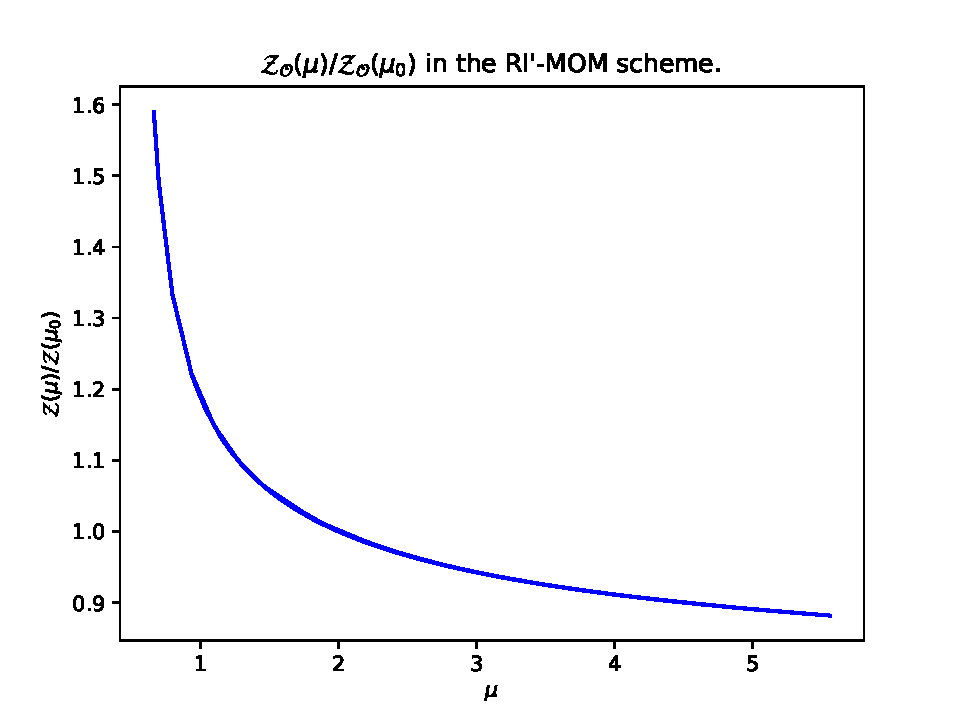
\includegraphics[width = .6\textwidth]{ratio_op}
	\caption{Ratio $\mathcal{Z}(\mu) / \mathcal{Z}(\mu_0)$ in the RI'-MOM scheme.} 
\end{figure}

To convert a R.C. given in RI'-MOM to $\overline{MS}$, we use Gracey's result for the matching coefficients, Equation 4.3 
of~\cite{gracey_zo}. This explicitly gives us:
\begin{equation}
	C_\mathcal{O}(a, 0) = \frac{\mathcal Z_{RI'-MOM}(\mu_0)}{\mathcal Z_{\overline{MS}}(\mu_0)}
\end{equation}
and we take $C_\mathcal{O}^{-1}$ to pass from the RI'-MOM scheme to the $\overline{MS}$ scheme. 

Using these pieces, we can explicitly convert the renormalization coefficients computed at scale $\mu$ to $\overline{MS}$:
\begin{equation}
	\mathcal{Z}_{\mathcal O}^{\overline{MS}}(\mu) = C_{\mathcal O}^{-1} \left(\frac{\mathcal Z(\mu_0)}{\mathcal Z(\mu)}\right)_{P.T.} \mathcal Z_\mathcal{O}^{RI'-MOM}(\mu)
\end{equation}
Our result for $\mathcal{Z}_{\mathcal O}^{\overline{MS}}$ is compiled in the following figure.
\begin{figure}[H]
	\centering
	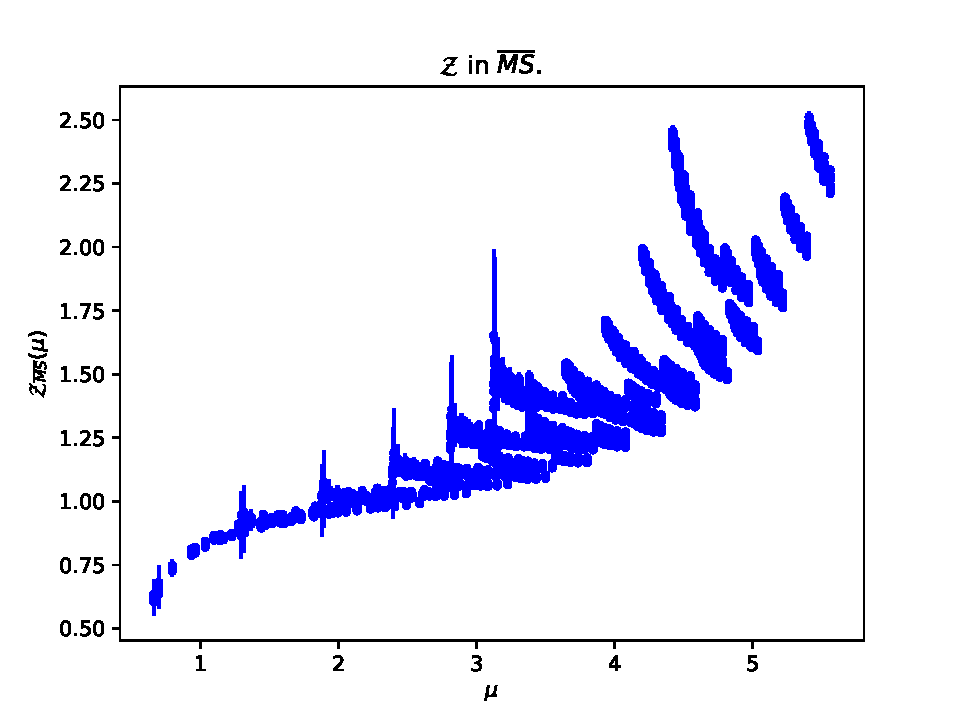
\includegraphics[width = .6\textwidth]{ZMSbar}
	\caption{$\overline{MS}$ renormalization coefficient.}
\end{figure}

\subsection{Fitting discretization artifacts}
\label{sec:artifacts}

When we compute observables at a finite lattice spacing $a$, we suffer \textbf{discretization artifacts} which are relics of the 
explicit symmetry breaking $SO(1, 3)\rightarrow H(4)$ suffered by putting the theory on a lattice. Namely, because we have 
less symmetry, there are more invariant quantities of $p^\mu$ in a lattice theory than in the continuum. In the continuum, the 
basic invariant that we can create is $p^2 = p_\mu p^\mu$. 

There are two basic types of discretization artifacts which will show up: artifacts from the breaking of Lorentz invariance 
$O(4)\rightarrow H(4)$, and artifacts from running. The symmetry breaking artifacts will appear in the data as ``fans". 
When these are removed, the data will appear to have a smooth structure, at which point one can solve for the running 
artifacts by expanding in all possible terms consistent with symmetry. 

To fit the artifacts from symmetry breaking, we may use the $\bf p^{[2n]}$ \textbf{extrapolation method}. This amounts to 
expanding the artifacts in a Taylor series in hypercubic invariants. 

On the lattice, we can find other invariants because the orbits of $H(4)$ are strictly smaller than the orbits of 
$O(4)$, the Euclidean isometry group in $d = 4$. For example, the vectors $(2, 0, 0, 0)$ and $(1, 1, 1, 1)$ have the same 
value of $p^2 = 4$, yet there is no element $g\in H(4)$ such that $g\cdot (1, 1, 1, 1) = (2, 0, 0, 0)$, i.e. they cannot be 
rotated into one another by hypercubic symmetry. This is because we can define \textit{other hypercubic invariants than 
just $p^2$}. The functions:
\begin{equation}
	p^{[2n]} := \sum_\mu p^{2n}
\end{equation}
for $n\in\mathbb N$ are also invariants, and these dictate the orbits of momenta under $H(4)$. Since $(1, 1, 1, 1)$ has 
$p^{[4]} = 4$ and $(2, 0, 0, 0)$ has $p^{[4]} = 16$, we can conclude they are distinct momenta under hypercubic 
symmetry and thus cannot live in the same orbit of $H(4)$. 

Any function which is invariant under the action of $H(4)$ must be a function of these hypercubic invariants, much like 
how in the continuum any function which was invariant under Lorentz symmetry was a function of Lorentz scalars like 
$p^2$ or $\slashed p$. Because we are computing out quantities on the lattice which only has $H(4)$ symmetry, these 
extra terms like $p^{[4]}$ can come into play when form factors or renormalization constants are computed, and this 
extrapolation method will account for these. 

Another source of error that we must consider when performing calculations on the lattice is that lattice momenta is quantized. 
The possible values that the momenta can take are:
\begin{equation}
	p_\mu = \frac{2\pi}{aL_\mu} k_\mu 
\end{equation}
where $k_\mu\in\mathbb Z$ and $L_\mu$ is the size of the lattice in direction $\mu$. In the lattice action, the momentum is 
modified to become:
\begin{equation}
	\tilde p_\mu = \frac{1}{a}\sin(ap_\mu)
\end{equation}
and in the small $a$ limit, notice that this reduces to the standard momentum values $p_\mu$. As a result, our renormalization 
coefficient computed on the lattice will be a function of $\tilde p_\mu$, \textit{not} a function of $p_\mu$. We wish to account 
for this and for our final result to be a function of $p_\mu$, so we must take this into account when fitting the hypercubic 
artifacts. 

TODO finish this section

\newpage
\thispagestyle{empty}

\begin{thebibliography}{99}

\bibitem{ri_mom}
Martinelli, G., Pittori, C., Sachrajda, C., Testa, M., Vladikas, A. (1994). A General Method for Non-Perturbative Renormalization of Lattice Operators arXiv https://dx.doi.org/10.1016/0550-3213(95)00126-d.

\bibitem{sergey}
Syritsyn, S. (2011). Exploration of Nucleon Structure in Lattice QCD with Chiral Quarks.

\bibitem{gockeler}
G\"{o}ckeler, M., Horsley, R., Nakamura, Y., Perlt, H., Pleiter, D., Rakow, P., Sch�fer, A., Schierholz, G., Schiller, A., St�ben, H., Zanotti, J. (2010). Perturbative and Nonperturbative Renormalization in Lattice QCD arXiv https://dx.doi.org/10.1103/physrevd.82.114511

\bibitem{gracey_zo}
Gracey, J. (2003). Three loop anomalous dimension of the second moment of the transversity operator in the MSbar and RI' schemes arXiv  667(1-2), 242-260. https://dx.doi.org/10.1016/s0550-3213(03)00543-1.

\bibitem{gracey_zq}
Gracey, J. (2003). Three loop anomalous dimension of non-singlet quark currents in the RI? scheme Nuclear Physics B  662(1-2)https://dx.doi.org/10.1016/s0550-3213(03)00335-3.

\bibitem{run_dec}
Herren, F., Steinhauser, M. (2017). Version 3 of {\tt RunDec} and {\tt CRunDec} arXiv  224(), 333-345. https://dx.doi.org/10.1016/j.cpc.2017.11.014.

\bibitem{pdg}
Tanabashi, M. \textit{et al}. (2018). Review of Particle Physics* Physical Review D  98(3), 030001. https://dx.doi.org/10.1103/physrevd.98.030001.

\end{thebibliography}

\end{document}